\documentclass[12pt]{beamer} %
\usepackage{amssymb,amsmath}
\usepackage[utf8x]{inputenc}
\usepackage{graphicx}
\setcounter{secnumdepth}{0}
\usetheme{Berkeley}
\usecolortheme{seagull}

\title[JBrowse as a Tool]{JBrowse as a Tool}
\author[E. Rasche]{E. Rasche}
\date{2015-07-07}
\usepackage{hyperref}


\begin{document}
\frame{\titlepage}

\section{What is it?}
\begin{frame}{JBrowse is a Genome Browser}
	\begin{itemize}
    	\item Fast
        \item Features! 
        \item Extensible
    \end{itemize}
\end{frame}

\subsection{Screenshots}



{
  \usebackgroundtemplate{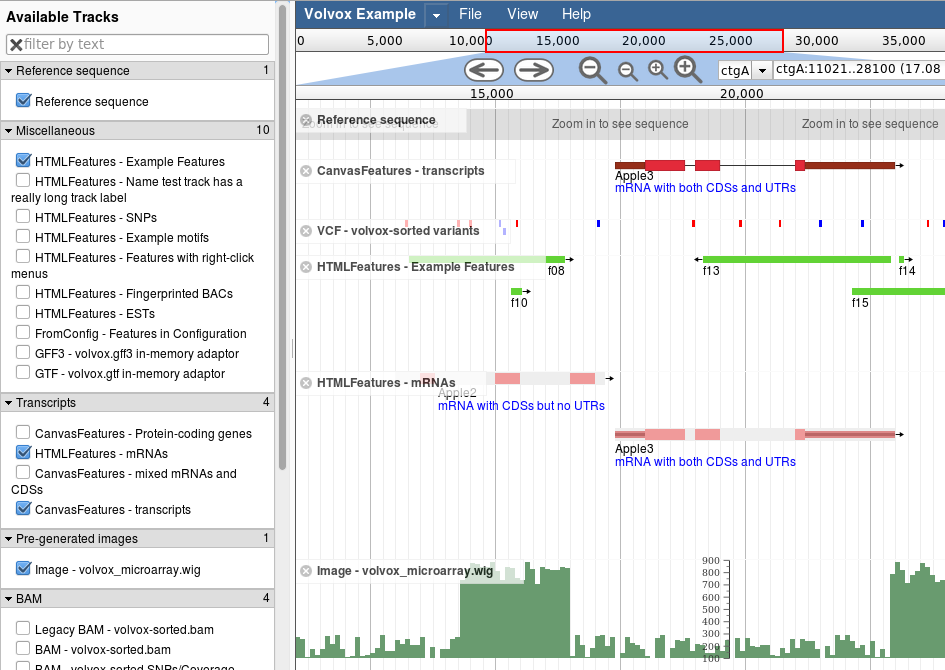
\includegraphics[height=\paperheight,width=\paperwidth]{snapshot10.png}}
  \setbeamertemplate{navigation symbols}{}
  \begin{frame}[plain]
  \end{frame}
}

{
  \usebackgroundtemplate{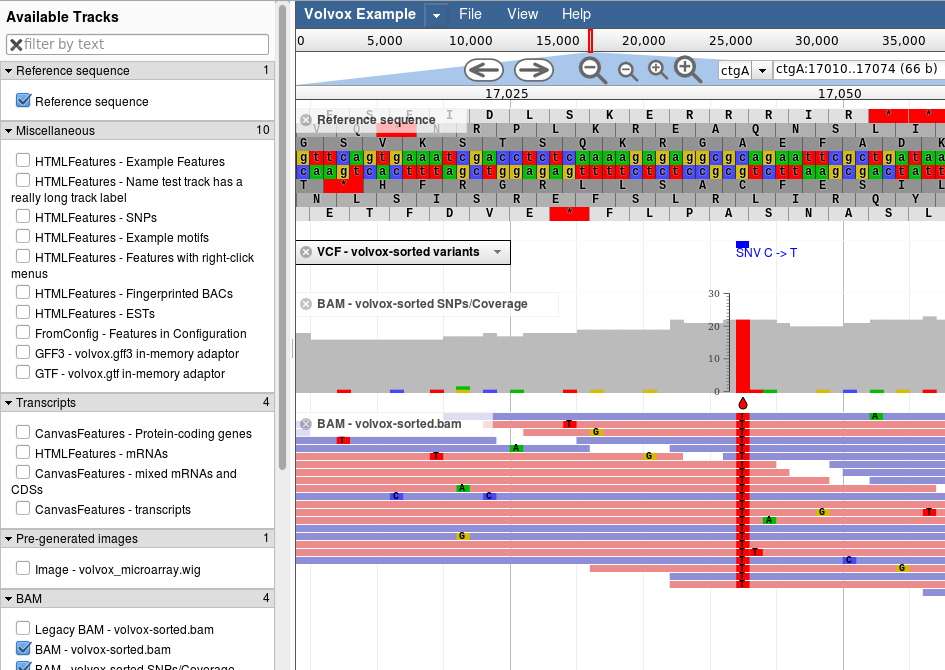
\includegraphics[height=\paperheight,width=\paperwidth]{snapshot11.png}}
  \setbeamertemplate{navigation symbols}{}
  \begin{frame}[plain]
  \end{frame}
}

\section{JBrowse in Galaxy}
\begin{frame}{Why JBrowse as a Tool? Workflows!}
	\centering
	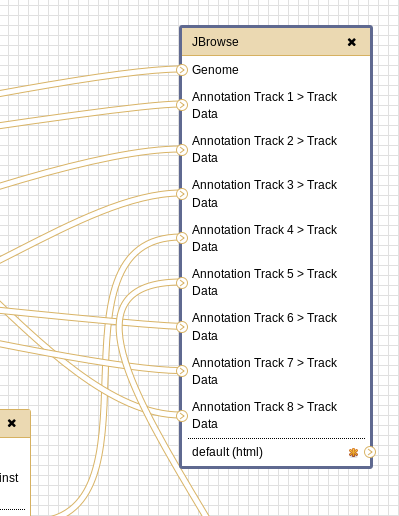
\includegraphics[width=\textwidth,height=0.8\textheight,keepaspectratio]{snapshot17.png}
\end{frame}


\section{Features}
\subsection{GFF3/BED}
\begin{frame}{GFF3/BED}
	\centering
	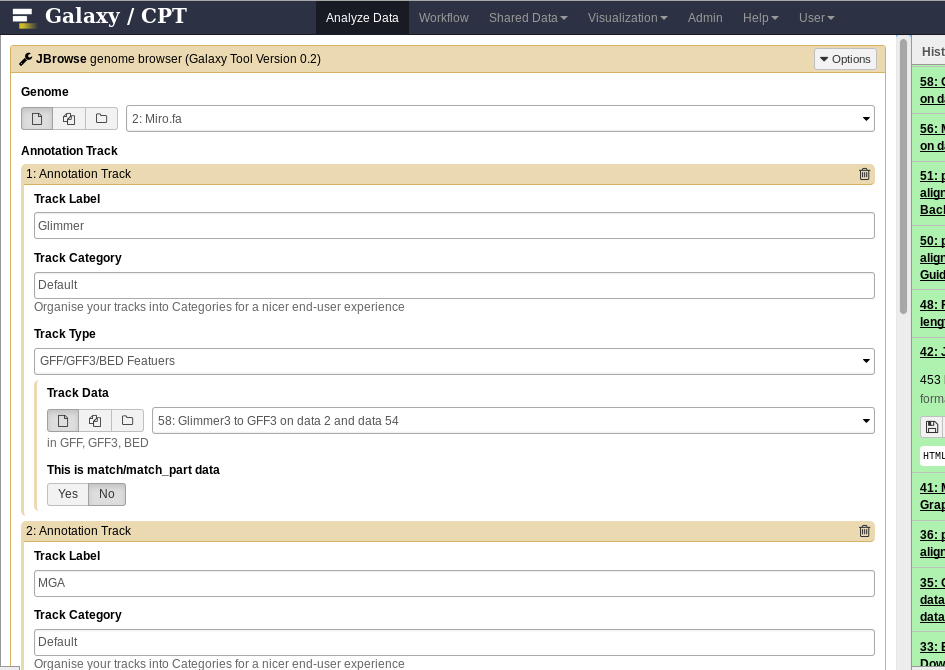
\includegraphics[width=\textwidth,height=0.8\textheight,keepaspectratio]{snapshot12.png}
\end{frame}

\subsection{BAM}
\begin{frame}{BAM}
	\centering
	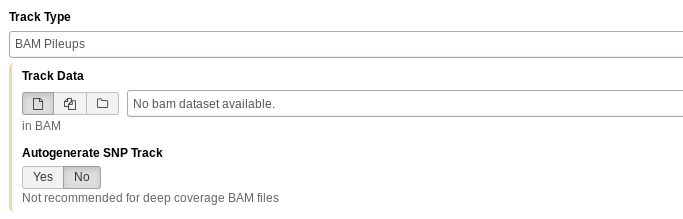
\includegraphics[width=\textwidth,height=0.8\textheight,keepaspectratio]{snapshot13.png}
\end{frame}

\subsection{Blast XML}
\begin{frame}{Blast XML}
	\centering
	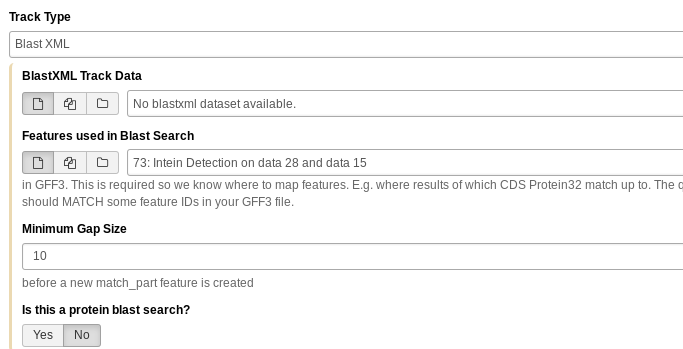
\includegraphics[width=\textwidth,height=0.8\textheight,keepaspectratio]{snapshot14.png}
\end{frame}

\begin{frame}{Gapped Blast XML}
	\centering
	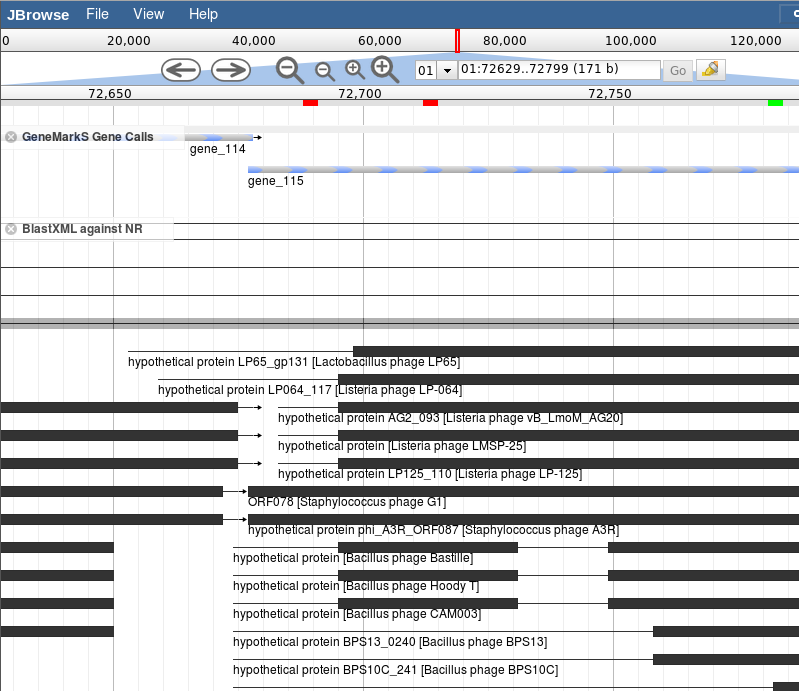
\includegraphics[width=\textwidth,height=0.8\textheight,keepaspectratio]{jb-blast.png}
\end{frame}

\subsection{BigWig}
\begin{frame}{BigWig}
	\centering
	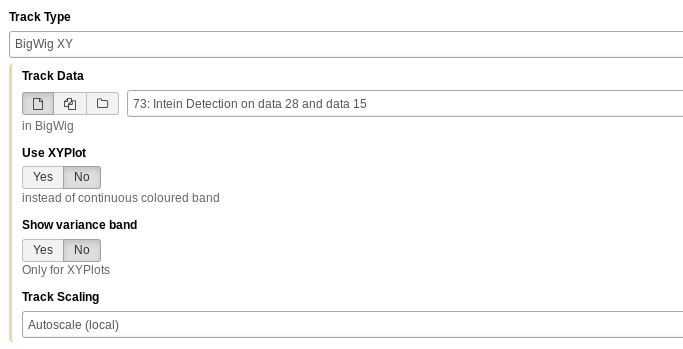
\includegraphics[width=\textwidth,height=0.8\textheight,keepaspectratio]{snapshot15.png}
\end{frame}

\subsection{VCF/SNPs}
\begin{frame}{VCF/SNPs}
	\centering
	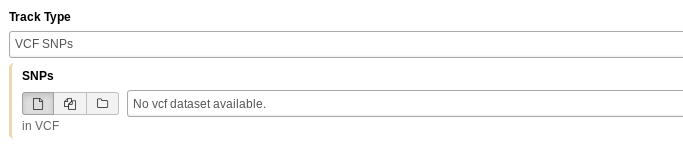
\includegraphics[width=\textwidth,height=0.8\textheight,keepaspectratio]{snapshot16.png}
\end{frame}

\section{Nice Features}
\begin{frame}{Nice Features}
	\begin{itemize}
        \item Lots of formats
        \item ``Sugar'' to support non-standard data for JBrowse like BlastXML
        \item Just an HTML dataset, download, view, deploy to production servers
    \end{itemize}
\end{frame}

\section{Roadmap}
\begin{frame}{Planned Features}
	\begin{itemize}
        \item Soon more raw JBrowse configuration
        \item Color/track styling implemented
        \item Will be easier to configure ``production'' JBrowse instances
    \end{itemize}
\end{frame}

\section{Caveats}
\begin{frame}{Caveats/TODOs}
	\begin{itemize}
    	\item This is still a \textbf{work-in-progress} (but it's close!)
        \item Still some bugs in dependencies \& their installation process
        \item Broken upstream perl modules, yay! 
        \item JBrowse-in-Galaxy will not display BAM/BigWig files if you aren't using \texttt{X\_SENDFILE} (but I think we can fix this)
    \end{itemize}
\end{frame}



\section{Q\&A}
\begin{frame}{Q\&A}
	\begin{itemize}
    	\item Development: \url{https://github.com/galaxyprojec/tools-iuc}
        \item Twitter: @Eric\_Rasche
        \item Bugs/feature requests welcome!
    \end{itemize}
\end{frame}

\end{document}
